
\documentclass[a4paper, 11pt]{report}
\usepackage[utf8]{inputenc}
\usepackage{titlesec}
\usepackage{fullpage} % changes the margin
\usepackage{amsmath}
\usepackage{amssymb}
\usepackage{graphicx} %package to manage images
\usepackage[linkcolor=red]{hyperref}
\usepackage{paralist}
\graphicspath{ {./images/} }

\begin{document}
\begin{titlepage}
\vspace*{0.7in}
\begin{center}
\begin{figure}[htb]
\begin{center}

\includegraphics[width=8cm]{univ_logo}
\end{center}
\end{figure}
\vspace*{0.3in}
\begin{Large}
\textbf{SOEN 6011 : SOFTWARE ENGINEERING PROCESSES} \\
\end{Large}
\vspace*{0.1in}
\begin{Large}
\textbf{SUMMER 2021} \\
\end{Large}
\vspace*{0.9in}
\begin{Large}
\textbf{SUPER CALCULATOR} \\
\end{Large}
\vspace*{0.9in}
\begin{Large}
\textbf{PROBLEM - 1} \\
Function Description \\
\end{Large}
\vspace*{0.9in}
\rule{80mm}{0.1mm}\\
\vspace*{0.1in}
\begin{large}
Authors \\
\vspace*{0.1in}
Rokeya Begum Keya\\
\vspace*{0.1in}
Kyle Taylor Lange\\
\vspace*{0.1in}
Sijie Min\\
\vspace*{0.1in}
Manimaran Palani\\ 
\vspace*{0.3in}
\date{\normalsize\today} 
\end{large}
\end{center}
\end{titlepage}

\tableofcontents
\newpage
\addcontentsline{toc}{section}{a) Description of Functions}
\section*{Description of Functions}
\section*{\centering{PROBLEM 1 - F2: $tan(x)$}}
\normalsize {SOEN 6011 - Summer 2021} \hfill \textbf{Rokeya Begum Keya} \\
\textbf{ Software Engineering Processes}  \hfill \textbf{40183615} \\
\hfill Repository address : https://github.com/Dakatsu/SOEN6011Calculator
\\
 \subsection*{ Tangent Function, $tan(x)$ } 
 \normalsize{$tan(x)$ is a trigonometric function which relate a right-angled triangle to ratios of two side lengths. In addition, it also uses to find the slope of a line. The tangent function is define as below: \[tan(x) = \frac{sin(x)}{cos(x)}\]}
 \
 \subsection*{Graph}
 \normalsize{In the graph of a tangent function, there are no high or low points, so this function does not have an amplitude.}
 \begin{center}
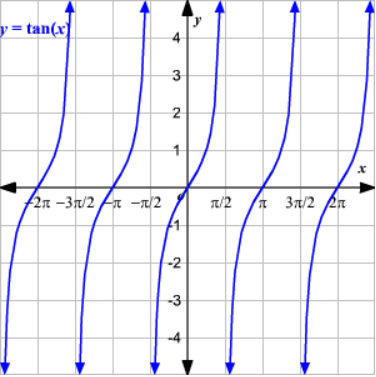
\includegraphics[width= 4cm]{tan}
\end{center}
\begin{center}
Graph of tangent function $y = tan(x)$\end{center}
 \normalsize{Where, $x$ is real number. The tangent function is undefined when $cos(x) = 0 $, therefore, tangent function has a vertical asymptote whenever $cos(x) = 0 $. }
 \subsection*{Range}
 \normalsize{ The range of $tan(x)$ is all real number (negative to positive infinity), except 0. The $tan(x)$ does not have amplitude therefore, it has vertical asymptotes. As, tangent function increases and decreases without bound between vertical asymptotes, there is no horizontal asymptotes exist for it.}
 
 \subsection*{Domain and Co-domain}
 \normalsize{The domain of tangent function is all real number except the value where $cos(x) = 0$ because if $cos(x) = 0$ then $tan(x)$ will be undefined. The co-domain of $tan(x)$ is \((-\infty, +\infty\)).}
\pagebreak

\section*{\centering{PROBLEM 1 - F3: Hyperbolic Sine, $sinh(x)$}}
\normalsize {SOEN 6011 - Summer 2021} \hfill \textbf{Kyle Taylor Lange} \\
\textbf{ Software Engineering Processes}  \hfill \textbf{27627696} \\
\hfill Repository address : https://github.com/Dakatsu/SOEN6011Calculator
\\\\\\\\\\
\normalsize{The function $sinh(x)$ is known as the hyperbolic sine, and it has the following formula \cite{sinh}. 
$$sinh(x) \equiv \frac{1}{2}(e^x-e^{-x})$$
The character $x$ is the only variable, as $e$ is a constant roughly equivalent to 2.71828 \cite{e}. Both the domain and co-domain of $sinh(x)$ is $\mathbb{R}$, i.e. (-$\infty$, +$\infty$). Positive values of $x$ trend toward +$\infty$, negative values of $x$ trend toward -$\infty$, and an input of 0 outputs 0.
\\Just as the trigonometric functions sine and cosine relate to a unit circle \cite{circular}, their hyperbolic equivalents relate to the right branch of a unit hyperbola \cite{hyperbolic}. The x-coordinate of the right branch of the hyperbola at a given hyperbolic angle $a$ can be calculated with $cosh(a)$, and $sinh(a)$ will return the y-coordinate \cite{rectHyperbola}.}
\begin{thebibliography}{}
\bibitem{sinh}
Hyperbolic Sine, Wolfram MathWorld.
\\http://mathworld.wolfram.com/HyperbolicSine.html
\bibitem{hyperbolic}
Hyperbolic Functions, Wolfram MathWorld.
\\http://mathworld.wolfram.com/HyperbolicFunctions.html
\bibitem{circular}
Circular Functions, Wolfram MathWorld.
\\http://mathworld.wolfram.com/CircularFunctions.html
\bibitem{e}
e, Wolfram MathWorld.
\\http://mathworld.wolfram.com/e.html
\bibitem{rectHyperbola}
Rectangular Hyperbola, Wolfram MathWorld.
\\https://mathworld.wolfram.com/RectangularHyperbola.html
\end{thebibliography}
\pagebreak

\section*{\centering{PROBLEM 1 - F*}}
\normalsize {SOEN 6011 - Summer 2021} \hfill \textbf{Sijie Min} \\
\textbf{ Software Engineering Processes}  \hfill \textbf{401*****} \\
\hfill Repository address : https://github.com/Dakatsu/SOEN6011Calculator
\\\\\\\\\\
 \begin{center} Team please add your content here \end{center}
\pagebreak

\newcommand{\R}{\mathbb{R}}
\renewcommand{\labelitemi}{$\star$}
\section*{\centering{PROBLEM 1 - F7 : \(x^y\)}}
\normalsize {SOEN 6011 - Summer 2021} \hfill \textbf{Manimaran Palani} \\
\textbf{ Software Engineering Processes}  \hfill \textbf{40167543} \\
\hfill Repository address : https://github.com/Dakatsu/SOEN6011Calculator
\subsection*{Definition of \(x^y\)}
\cite{mathInsight} Exponentiation is a mathematical operation, denoted as \(x^y\), If y is a positive integer and \(x\) is any real number, then \(x^y\) corresponds to repeated multiplication.
 \begin{center} \(x^y\) = \(x\)*\(x\)*\(x\)*.....*\(x\) of y times \end{center}
The expression can be called as “\(x\) raised to the power of y,” “\(x\) to the power of y,” or simply “\(x\) to the y.” Here, \(x\) is the base and y is the exponent or the power.
\subsection*{Domain}
\cite{mathbits} All the real numbers from -infinite to +infinite.(-\(\infty\) to \(\infty\))
 \begin{center} $(x,y) \in \R^2 : (x \geq 0 \land y \neq 0) \lor x>0$ \end{center}
\subsection*{Co-domain}
A set of all positive real numbers from zero to infinite (0 to \(\infty\)) is known as the Exponentiation function
\subsection*{Characteristics}
\begin{flushleft}
\textbf{Graph - }
 \end{flushleft}
\begin{flushleft}
\cite{mathbits}\cite{wolframalpha} The \textbf{rate of change} increases (or decreases) across the graph in an exponential graph.
\end{flushleft}
\begin{itemize}
\item \label{graph} The exponential graph crosses the y-axis at (0,1). 
\item The exponential graph increases, when x \(>\) 1.
\item The exponential graph decreases, when 0 \(<\) x \(<\) 1.
\item The exponential graph is asymptotic to the x-axis - gets very, very close to the x-axis but, in this case, does not touch it or cross it.
\end{itemize}
\begin{center}
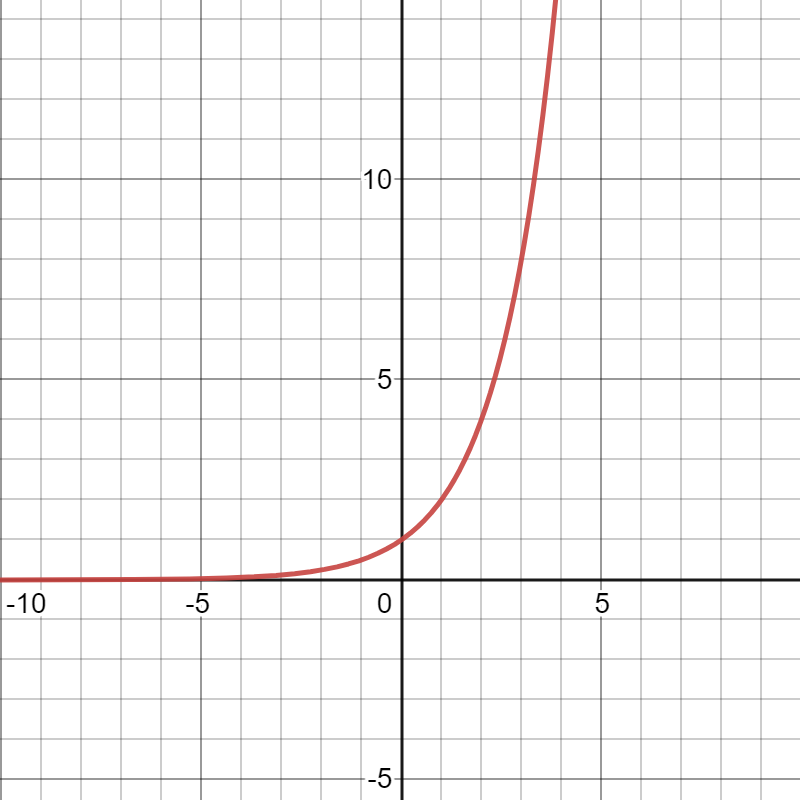
\includegraphics[width=5cm]{x^y}
\end{center}
\begin{center}
Graph crosses the y-axis at (0,1)\end{center}
\begin{thebibliography}{}
\bibitem{mathInsight} 
Nykamp DQ: Basic rules for exponentiation
\\\texttt{https://mathbitsnotebook.com/Algebra2/Exponential/EXExpFunctions.html}
\bibitem{mathbits} 
MathBits Teacher: Exponential Functions,
\\\texttt{https://mathbitsnotebook.com/Algebra2/Exponential/EXExpFunctions.html}
\bibitem{wolframalpha} 
WolframAlpha: Domain of exponentiation function,
\\\texttt{https://www.wolframalpha.com/input/?i=x\%5Ey}
\end{thebibliography}
\newpage
\addcontentsline{toc}{section}{b) Context of Use Model}
\section*{Context of Use Model}
\begin{center}
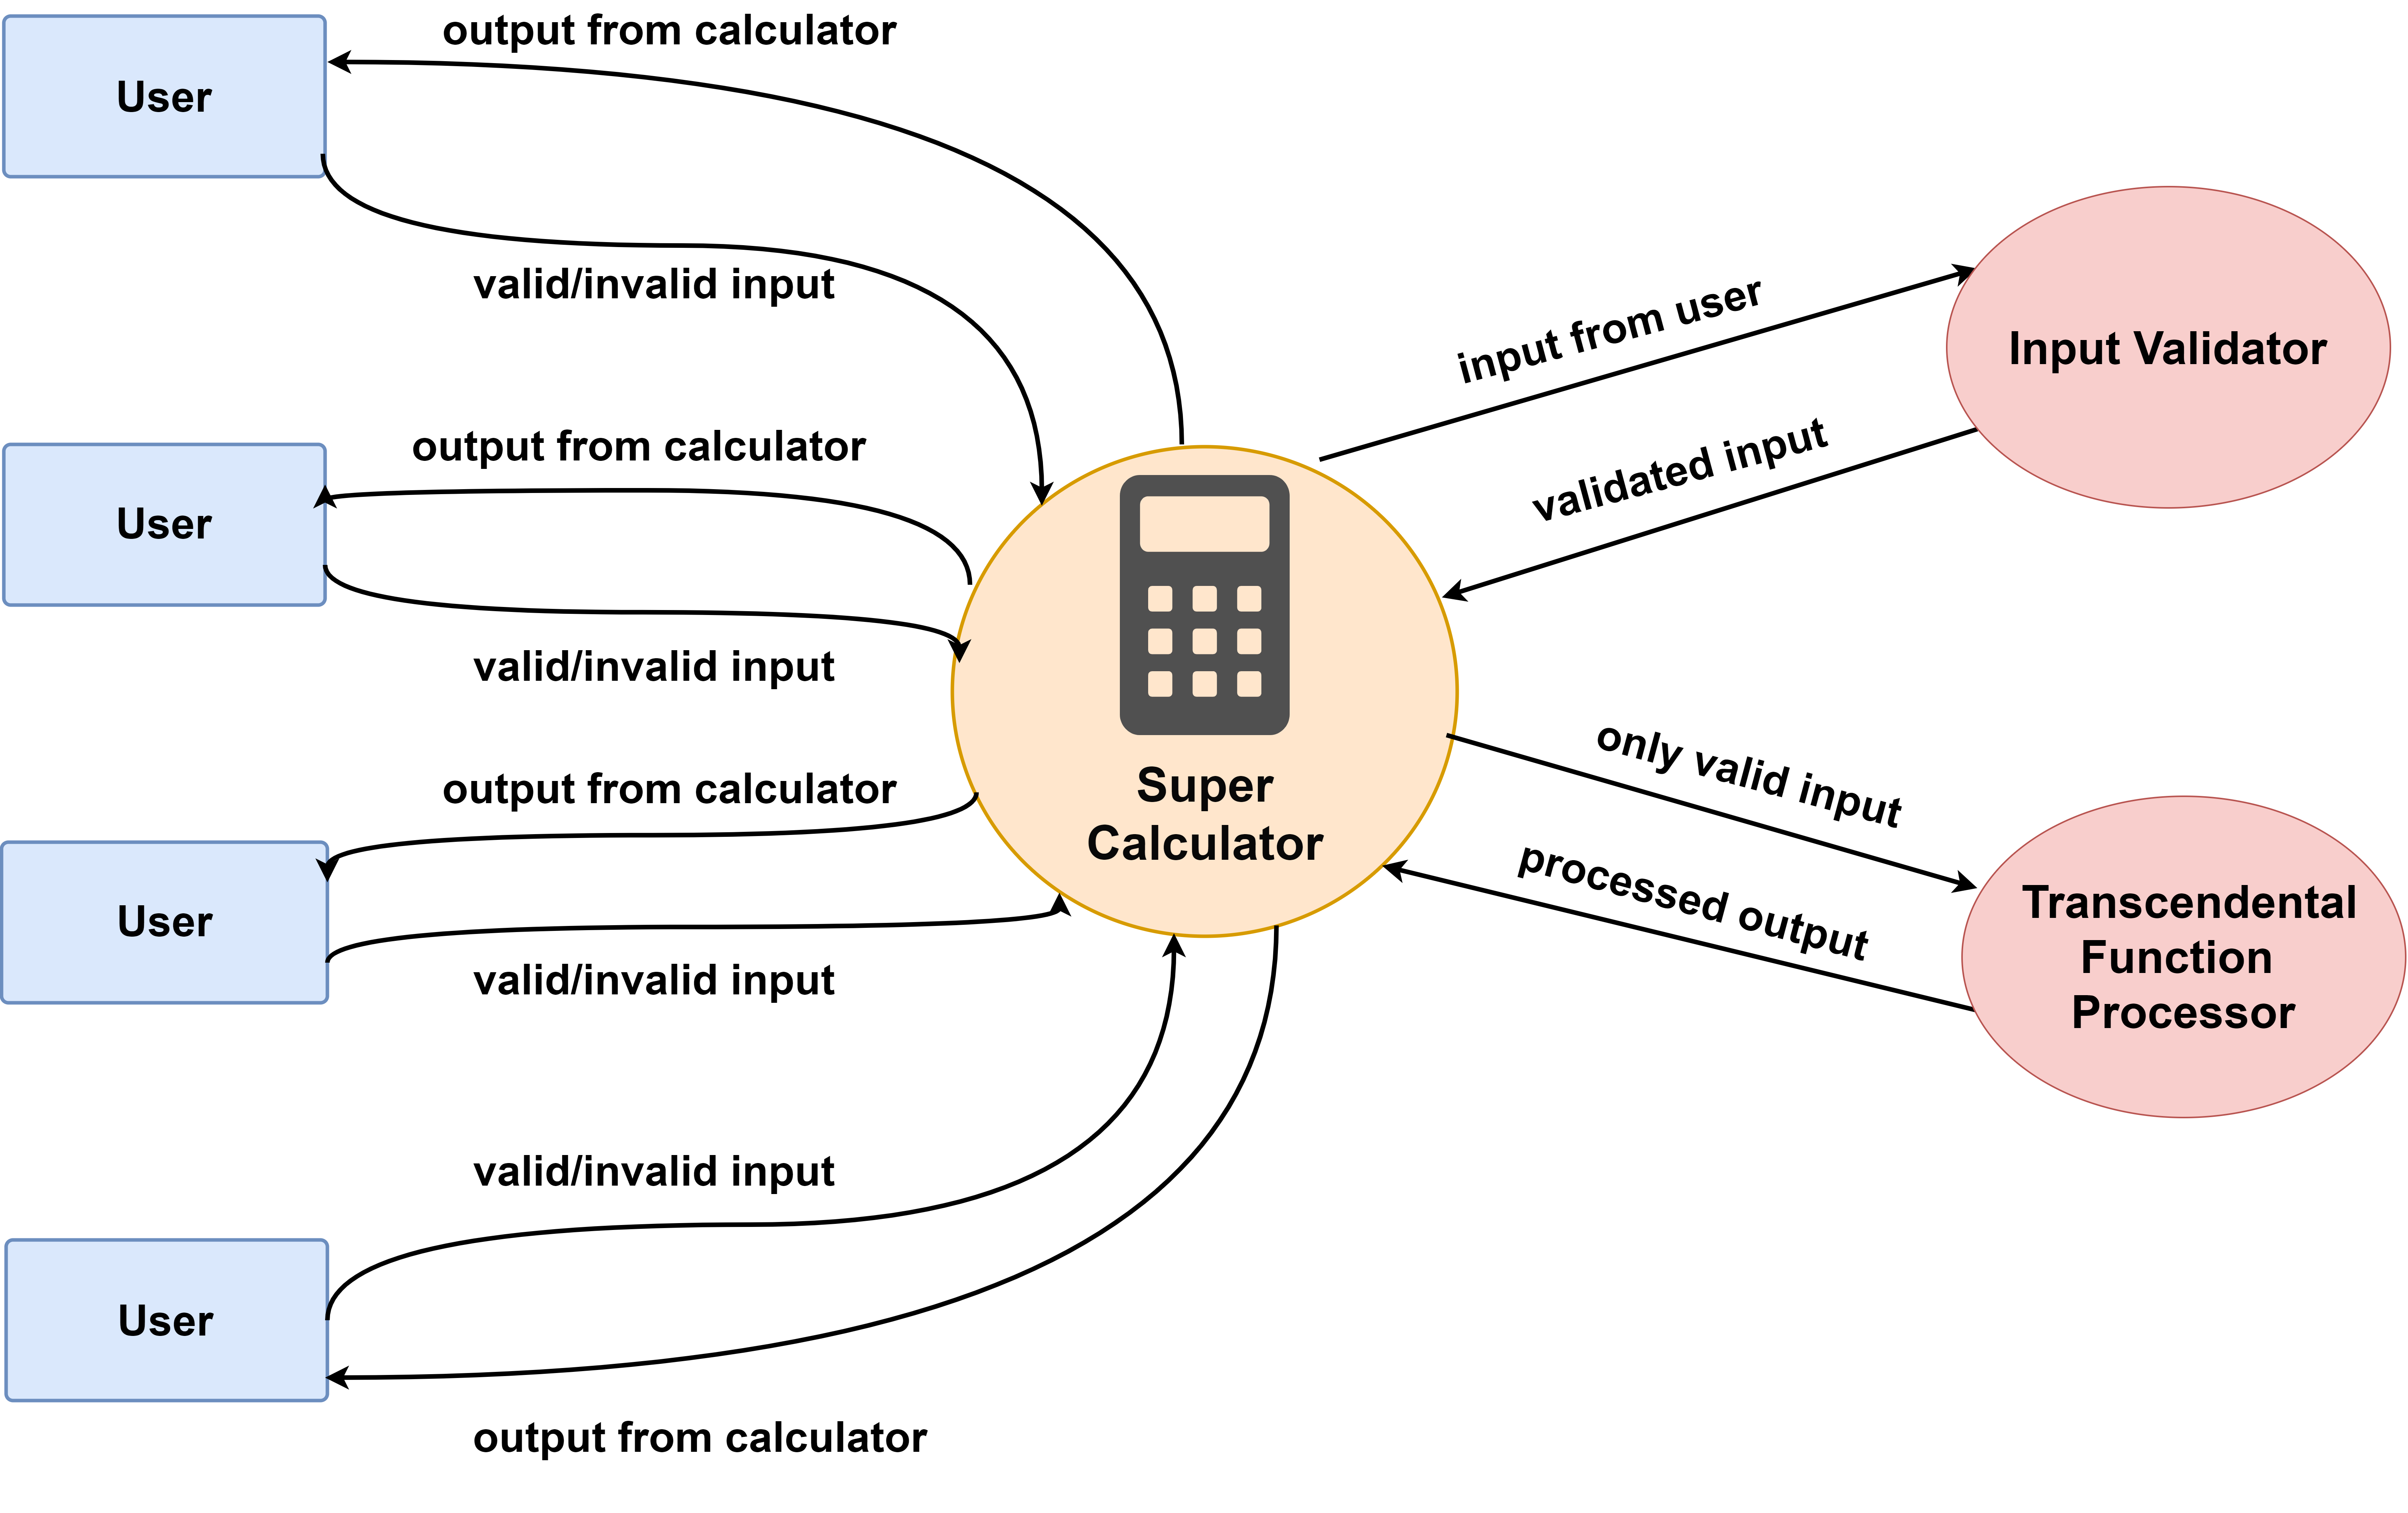
\includegraphics[width=15cm]{context_diagram}
\end{center}
\end{document}
